\documentclass{article}
\usepackage[utf8]{inputenc}
\usepackage{amsfonts}
\usepackage{amssymb}
\usepackage{graphicx}
\usepackage{hyperref}
\usepackage{amsmath}
\usepackage{pgfplots}
\pgfplotsset{compat=1.18}
\usepackage[backend=biber, style=numeric]{biblatex}
\addbibresource{references.bib}
\usepackage{titlesec}
\titleformat{\subsection}[hang]{\normalfont\bfseries}{\thesubsection}{1em}{}
\usepackage{abstract}
\usepackage[labelformat=empty]{caption}

\begin{document}
\pagenumbering{gobble}
\begin{figure}
  \centering
  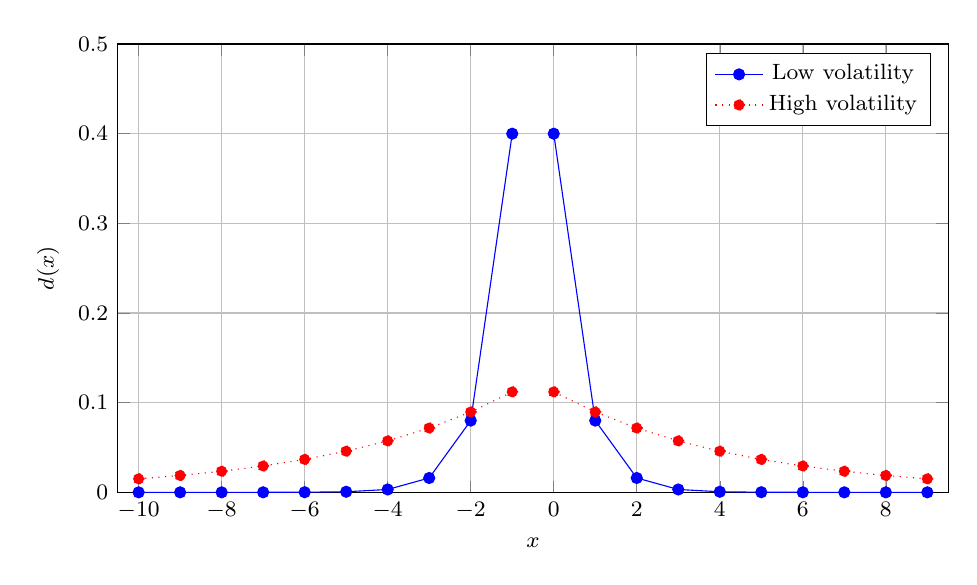
\begin{tikzpicture}
    \begin{axis}[
      xlabel={$x$},
      ylabel={$d(x)$},
      xmin=-10.5, xmax=9.5,
      ymin=0, ymax=0.5,
      xtick={-10,-8,-6,-4,-2,0,2,4,6,8,10},
      ytick={0,0.1,0.2,0.3,0.4,0.5},
      grid=major,
      width=\columnwidth,
      height=0.6\columnwidth,
      tick label style={font=\footnotesize},
      label style={font=\footnotesize},
      legend style={font=\footnotesize},
    ]
    
    \addplot[domain=-10:-1, samples=10, color=blue, mark=*]{0.5 * 0.2^(-(x+1)) / ((1 - 0.2^10) / (1 - 0.2))};
    \addlegendentry{Low volatility}

    \addplot[domain=-10:-1, samples=10, color=red, mark=*, dotted]{0.5 * 0.8^(-(x+1)) / ((1 - 0.8^10) / (1 - 0.8))};
    \addlegendentry{High volatility}

    \addplot[domain=0:9, samples=10, color=blue, mark=*]{0.5 * 0.2^x) / ((1 - 0.2^10) / (1 - 0.2))};

    \addplot[domain=0:9, samples=10, color=red, mark=*, dotted]{0.5 * 0.8^x) / ((1 - 0.8^10) / (1 - 0.8))};
    
    \end{axis}
  \end{tikzpicture}
  \caption{LDF for a major volatile pair (e.g. ETH/USDC). Liquidity concentration decreases when volatility increases.}
  \label{fig:major_volatile}
\end{figure}

\end{document}